\documentclass{article}

\usepackage{amsmath}
\usepackage{amssymb}
\usepackage{graphicx}
\usepackage{color}

\begin{document}
\section{Notation}
\textbf{$p_i$} is the ith patch.\\
\textbf{$f_{ij}$} is the fold line between $p_i$ and $p_j$.\\
\textbf{$Sf_i$} is the set of fold lines of $p_i$. Inside this set, fold lines are sorted by their x position.\\
\textbf{$x(f_{ij}$)} is the x position of fold line $f_{ij}$.

\section{Formulation}
First find one fold line between each pair of patches. Then get $Sf_i$ through the following steps:
\begin{enumerate}
\item
  Collecting all fold lines on $p_i$.
\item
  Sort these fold lines based on x position.
\item
  Insert one fold line between each neighbor pair of fold lines. We call one new added fold line $f_i^k$, indicating its the kth new added fold line on $p_i$.
\end{enumerate}
After finding all possible fold lines, we try to assign one binary indicator $i(f)$ for each fold line indicating whether it should be kept or not. If $i(f)$ equals to 1, f will be kept, and if $i(f)$ equals to 0, f will be discarded.

So, we want to minimize the function $g(I)$:
\begin{equation}
  g(I) = \sum{D(i(f))}
\end{equation}
Here $D(i(f))$ is the data term in the following form:
\begin{equation}
  D(i(f)) = 
  \begin{cases}
    data \quad cost \quad for \quad f \quad if \quad i(f) = 1\\
    0 \quad if \quad i(f) = 0
  \end{cases}
\end{equation}
The data cost for f can be calculated based on some input information, curvature of the boundary for example.

\color{red}
The optimization also subjects to some constraints. To avoid orientation conflict, i.e. to ensure each patch has a fixed orientation, we need to add constraints in the following way:
\begin{enumerate}
\item
  For $p_i$, find all paths starting from background patch (the left one) to $p_i$.
\item
  Represent path k using the fold lines it pass through as $P^k = \{f_1^k, f_2^k, ...\}$.
\item
  Then for each pair of paths $P^s$ and $P^t$, there is constraint $\sum_i(i(f_i^s)) + \sum_i(i(f_i^t)) = an \quad even \quad number$. This means these two values are both either odd or even, indicating the same direction for $p_i$. However, I don't have experience about constraints like this.
\end{enumerate}
\color{black}

% There is another type of constraints which ensures that there would be a path passing through each patch. The constraints can be enforced in the following way. For $p_i$, find all $f_{ij}$ lying on the left side of $p_i$ and enforce that the sum of their indicators is greater than 1. Do the same with fold lines lying on the right side of $p_i$.

\subsection{Fold Line Position Optimization}
To determine fold line positions together with fold line indicators, we can change the energy function by the following.
\subsubsection{New Constraints}
For each patch $p_i$, use an indicator $O(p_i)$ to determine whether the patch has even order or odd order. $O(p_i)$ takes a value of 0 or 1 and subjects to the following constraint.

\color{red}
(Previous equation about $O(p_i)$:
\begin{equation}
  \sum_j{i(f_j)} + O(p_i) = 2k
\end{equation}
The summation of fold line indicators consider one path from the background patch to $p_i$.
)
\color{blue}

Note that for an inactive fold line, it has two possible outcomes: to be cut (two patches becomes disconnected) and to flattened (two patched are merged into one), so we need another set of binary indicators $c(f)$ indicating whether $f$ is cut or not ($c(f) = 1$ means $f$ is cut). For fold lines added inside an initial patch, $c(f)$ is always $0$. For other fold lines, we might add a penalty for $c(f)$ based on geometry. (Take the bear for example, the fold line between the arm and the body prefer to be flattened while the fold line between the arm and the leg is more likely to be cut.) Also $c(f)$ should be $0$ when the fold line is active ($i(f) = 1$), so there is $c(f) <= 1 - i(f)$. Now we determine $O(p)$ by considering neighboring patches. $O(p_b) = 0$ ($p_b$ is the left background patch) holds for sure. Then for two neighboring patches $p_i$ and $p_j$ connected by fold line $f$, there is:
\begin{equation}
  (O(p_i) + i(f))(1 - c(f)) = (2k + O(p_j))(1 - c(f))
\end{equation}
If $f$ is active ($i(f) = 1$), then the order of $p_i$ and $p_j$ should be different. When $f$ is flattened ($i(f) = 0$ and $c(f) = 0$, the order between $p_i$ and $p_j$ should be same. If $f$ is cut ($i(f) = 0$ and $c(f) = 1$), then the order between $p_i$ and $p_j$ have no relation.

Note that this also determines fold line orientations, so we actually no longer need fold line orientation constraints.

\color{black}

\begin{figure}[h]
  1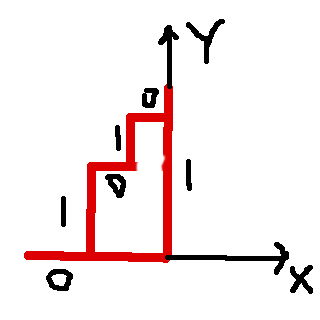
\includegraphics[width = 5cm, height = 5cm]{Figures/coordinates}
  \caption{Coordinates and examples of O(p)}
  \label{fig: Coordinates}
\end{figure}

We use $X(f)$ and $Y(f)$ for each fold line to indicate its 3D position. And for any pair of fold lines, $f_s$ and $f_t$, on $p_i$ there are constraints like (suppose $f_s$ lies left to $f_t$ on image):
\begin{multline}
  X(f_s)O(p_i) = X(f_t)O(p_i)\\
  Y(f_s)(1 - O(p_i)) = Y(f_t)(1 - O(p_i))\\
  X(f_s)(1 - O(p_i)) < X(f_t)(1 - O(p_i))\\
  Y(f_s)O(p_i) < Y(f_t)O(p_i)
\end{multline}
Note that since $O(p_i) = 0 \quad or \quad 1$, two of the above constraints are actually dummy.

\subsubsection{New Terms in Objective Function}
We can add some new terms in objective function to optimize fold line positions. We add some cost for fold line f like this:
\begin{equation}
  C(f) = (X(f) + Y(f) - x_f)^2
\end{equation}
$x_f$ is the original position of $f$ on image domain which is a given value and $X(f) + Y(f)$ is the new position of $f$ on image domain. Note that we do not need to distinguish active fold lines and inactive fold lines here for simplicity.

\subsection{Stability}
To consider stability, we add a set of binary variables $a_{ij}$, which indicates whether patch $p_i$ and patch $p_j$ are directly connected. A set of variables $b_{ij}$, which indicates patch $p_i$ and patch $p_j$ share common neighbors. $b_{ij}$ can take value from \{0, 1, 2\}. $b_{ij} = 0$ means two patches don't share any common neighbor. $b_{ij} = 1$ means two patches share one common neighbor (or one patch has a neighbor who is double connected with another patch). $b_{ij} = 2$ means two patches share at least two common neighbors. A set of binary variables $s_{i}$ which indicate whether a patch is stable or not.

\subsubsection{New Terms in Objective Function}
Add some penalties to encourage $a_{ij}$ to be zero if there is no constraint:\\
$\sum_{ij}a_{ij}$\\
Add some penalties to encourage $b_{ij}$ to be as large as possible:\\
$\sum_{ij}{2 - b_{ij}}$\\
Add some penalties to encourage $s_{i}$ to be one:\\
$\sum_{i}(1 - s_i)$\\
% Add some penalties to encourage $d_{i}$ to be one:\\
% $\sum_{i}(1 - d_i)$\\

\subsubsection{New Constraints}
Define $N(i)$ as the set of neighbor patches of $p_i$.\\
For patches $p_i$, $p_j$ and $p_k$:
$a_{jk} = f_{jk}$\\ which means if $f_{jk}$ is active, $p_j$ and $p_k$ are directly connected.\\
$b_{ik} \leq \sum_{j \in N(k)}{a_{ij}}f_{jk}$. The summation equals to the number of common neighbors $p_i$ and $p_k$ have.\\
(Note that in order for $p_i$ and $p_k$ to have common neighbor, they should not be the same patch or two connected patches, so there is $b_{ii} = 0$ and $b_{ik} = 0$ if $p_i$ and $p_k$ are directly connected.)\\
% $b_{ij} + 1 \geq b_{ik}$ which simply say that $b_{ij}$ should be one if $b_{ik} = 2$.\\

For patch $p_i$, there is:\\
\begin{equation}
  1.5 * s_i \leq \sum_j{a_{ij} * s_j} + \sum_j{b_{ij} * s_j} \times 0.5
  \label{eq:stability}
\end{equation}

This basically says that a patch is stable if:
\begin{enumerate}
\item It is connected with two or more stable patches. ($\sum_j{a_{ij} * s_j} \geq 2$)
\item It is connected with one stable patch and shares common neighbors with another stable patch.
\item It shares common neighbors with at least three stable patch.
\item It is double connected with one stable patch and shares common neighbors with another stable patch.
\end{enumerate}

And if $f_{ij}$ is flattened ($i(f_{ij}) = 0$ and $c(f_{ij}) = 0$), then $p_i$ and $p_j$ are the same patch, so there is:
\begin{enumerate}
\item $s_i(1 - i(f_{ij}) - c(f_{ij})) = s_j(1 - i(f_{ij}) - c(f_{ij}))$
\item $a_{ik}(1 - i(f_{ij}) - c(f_{ij})) = a_{jk}(1 - i(f_{ij}) - c(f_{ij}))$
\item $b_{ik}(1 - i(f_{ij}) - c(f_{ij})) = b_{jk}(1 - i(f_{ij}) - c(f_{ij}))$
\end{enumerate}

\color{blue}
Problem arises as the stability of a patch is usually established by the support of some other stable patches. That is to say, like connectivity, stability also has the concept of ordering (two background patches are stable initially, and then some patches become stable because of background patches, and some other patches becomes stable and so on). Current problem is that two or more patches lie to each other claiming that they are stable and support each other. Then they think they have enough support to be stable. The fact is, one of them has to become stable before it can provide support to others. So we have to model this ordering constraint somehow. So we use $s_{ik}$ to indicate whether a patch is stable with order $k$. The order is defined such that background patches have order $0$ and patches which become stable because of existing stable patches have an order greater than the order of existing stable patches. The formulation does not change much. The single equation \ref{eq:stability} becomes a set of equations, one for each order:
\begin{equation}
  1.5 * s_{ik} \leq \sum_j(a_{ij} \sum_{l=1}^{k-1}s_{jl}) + 0.5\sum_j(b_{ij} \sum_{l=1}^{k-1}s_{jl})\\
\end{equation}
Add constraints to ensure each patch is stable $\sum_k{s_{ik}} = 1$ (the term corresponding to $s_i$ becomes useless if constraints are added). Note that the maximum order $k$ could be quite large (around $\frac{number of patches}{2}$), but often it is small. So we can set $5$ as the maximum number of $k$, which means we only use $5$ indicators for each patch to make our problem tractable.
\color{black}

\subsection{Connectivity}
With background patches, every patch are connected, so background patches and fold lines lying on background patches are excluded from consideration. Then we select one patch $p_s$ arbitrarily and claim that every other patch has a path to $p_s$ and the length of this path is $d$. We know that $d \leq \# patches - 3$ (two background patches and $p_s$ are excluded. So we define a set of binary variables $d_{in}$ indicating $p_i$ has a path to $p_s$ with length n.\\
\color{red}
Here we define another set of indicators $f'_{ij}$ based on $f_{ij}$ such that $f'_{ij} = 1$ if $f_{ij}$ is added in the middle of an initial patch and $f'_{ij} = f_{ij}$ if $f_{ij}$ is added between two initial patches. The intuition here is to use $f'_{ij}$ to indicate whether $p_i$ and $p_j$ are connected. And for the first case, two patches are always connected regardless of the fold line between them since they come from one initial patch.\\
\color{blue}
Here, $f'_{ij}$ could be replaced by $c(f)$.
\color{black}

We then have:\\
$d_{i1} = f'_{is}$ (for neighbor patches of $p_s$) which means $p_i$ has a path to $p_s$ with length 1 only when it is connected with $p_s$.\\
$d_{in} \leq \sum_{j \in N(i)}{d_{j(n-1)}f'_{ij}}$ which means $p_i$ could have a path to $p_s$ with length n only when at least one of its neighbor patch has a path to $p_s$ with length n - 1.\\
For global connectivity, every patch should have a path to $p_s$, so $\sum_{n=1}^{max\_length}{d_{in} \geq 1}$ should be true for every patch except two background patches and $p_s$.

\subsection{Main fold line}
Main fold line may not be necessary. We only need to put a fold line between two background patch. Besides, we add two sets of constraints in the same manner with the fold line position constraints. This time constraints are enforced on each pair of fold lines lying on the same background patch.

\subsection{User interaction}
There are several possible user requirements:
\begin{enumerate}
\item \textbf{Symmetry} Divide the graph into two by the main fold line and consider only half of the graph. (I think the main fold line is special only in this case.)
\item \textbf{Patch Orientation (e.g. The nose should extrude out.)} Add a constraint $O(p) = 1 (or 0)$.
\item \textbf{Fold Line Status and Position} User might want to enforce a fold line to be active, flattened or cut. Or user might want to restrict a fold line's position. These requirements can be added to our formulation by adding corresponding constraints.
\item \textbf{New Fold Lines or Patches} User might want to add a new fold line or a new patch somewhere. We can easily modify our graph for this.
\end{enumerate}

\end{document}